
% JuliaCon proceedings template
\documentclass{juliacon}
\setcounter{page}{1}

%%%
%% Language Support
%%%
\usepackage[english]{babel}
\usepackage{csquotes}

%%%
%% Images
%%%
\usepackage{graphicx}
\graphicspath{{figures/}}
\usepackage[export]{adjustbox}

%%%
%% Fonts and Typewriting
%%%
\usepackage{mathtools}
\usepackage{amssymb}
\usepackage{bbm}
\usepackage{bm}
\usepackage{microtype}

%%%
%% Enhances Figures and Tables environments
%%%
\usepackage{placeins}
\usepackage[hypcap=true]{caption}
%\captionsetup[table]{labelfont=bf,textfont=it}
%\captionsetup[figure]{labelfont=bf,textfont=it}
\usepackage{booktabs, multirow, array, tabularx, floatrow, cellspace, threeparttable}
\floatsetup[table]{capposition = top}
\newcolumntype{Z}[1]{>{\centering\arraybackslash}p{#1}}
\newcolumntype{Y}{>{\centering\arraybackslash}X}
\renewcommand{\arraystretch}{1.25}

%%%
%% Enables hyperlinks
%%%
\usepackage{varioref}
\hypersetup{
    pdftitle    = {Econometrics.jl},
    pdfsubject  = {JuliaCon 2019 Proceedings},
    pdfauthor   = {José Bayoán Santiago Calderón},
    pdfkeywords = {Julia, Econometrics, Statistical Software, Software Validation},
    colorlinks  = true,
    linkcolor   = black,
    filecolor   = black,
    urlcolor    = black,
    citecolor   = black
}
\urlstyle{same}

\begin{document}

% **************GENERATED FILE, DO NOT EDIT**************

\title{My JuliaCon proceeding}

\author[1]{1st author}
\author[1, 2]{2nd author}
\author[2]{3rd author}
\affil[1]{University}
\affil[2]{National Lab}

\keywords{Julia, Optimization, Game theory, Compiler}



\maketitle

\begin{abstract}

% An abstract with at most 600 characters, written in plain English with no symbol nor formula.
% A list of at most 10 keywords as specified in the template, separated by commas and written in plain English.
% Compared to an extended abstract, a full paper presents more of the background and context motivating the work. It compares the work to other approaches taken in the field and gives some additional insights on the talk. Use cases back up the work by showing how it can be used.

Econometrics.jl is a package for econometrics analysis. It provides a series of most common routines for applied econometrics such as models for continuous, nominal, and ordinal outcomes, longitudinal estimators, variable absorption, weights, rank deficient, and robust variance covariance estimators.

\end{abstract}

\section{Introduction}

This study will: (1) provide an overview of common routines and their statistical and technical requirements, (2) provide an overview of tools available with their peculiarities, (3) discuss design decisions in the development of these tools, and (4) showcase \textit{Econometrics.jl} as a new tool for applied work.

Regression models may be used for several purposes. These may provide a basis for prediction models, causal inference, etc. Common targets include confidence intervals of the parameters estimates, joint-significance of a feature, out-of-sample predictive performance, and others. In other words, obtaining the estimates of a model is usually only part of the task. In order to judge a model, one may require to perform diagnostics and tests to justify potential conclusions for an analysis.

Regression analysis is at the core of applied econometrics. It can be challenging to grasp the extent what makes up the broad term of regression analysis. The following describes a very brief survey of what this technique might entail. Regression analysis can be used for both observational and experimental settings and it allows great flexibility for a multitude of applications. The main idea is to find estimates for model parameters to optimize some objective such as the likelihood in maximum likelihood estimation (MLE). Other potential objectives include restricted maximum likelihood (REML) or a Bayesian approach such as maximum a posteriori probability (MAP). One framework is the generalized linear model (GLM) which use a linear predictor that is mapped through a link function to a distribution modeling the response. Continuous responses might use a Normal distribution, count responses a log link with a Negative Binomial distribution, and probability models might use a categorical distribution with links that map to valid probabilities such as the Logit link. In cases such as probability models where the responses are multidimensional, the generalization is known as vector generalized linear models (VGLM). Other generalizations include relaxing the relation between the linear predictor and the outcome to be the sum of smoothing functions through a generalized additive model (GAM) framework or incorporating random effects through a mixed models approach. Some estimators address challenges such as endogeneity, censored responses, and zero-inflated responses through various solutions such as instrumental variables or censored regression model. Others, exploit aspects of the data to overcome challenges or increase efficiency such as random effects in longitudinal data. In relation to the second moment of the estimator, robust variance covariance estimators or boostrapping may be required for inference.

Out of the many potential tools practitioners may require, what are some of the most common? Not every estimator is as widely accessible or commonly used. Some educated guesses may be well justified such as ordinary least squares being more widely used than spatially-weighted regressions. In order to avoid speculation, I defer to a reasonable assumption that the most common estimators are those usually taught in academic programs and available in widely used software similarly to \cite{Renfro_2009}. Most programs teach tools to address the most common response types: continuous, count, rates, nominal, and ordinal outcomes. Hence, some routines might be linear models, Poisson/negative binomial, multinomial logistic regression, and ordinal logistic regression with proportional odds assumption. Topics in time series and panel data are usually offered in most programs. Perhaps the most common topic is short panels (many units of observations through relatively small number of repeated observations). Common estimators include pooling, first-difference, fixed effects / within estimator, and one-way random effects. The between estimator is usually masked as an intermediate model for estimating the error component in the random effects model. Lastly, the two big challenges taught in most programs are endogeneity and heteroscedasticity. These challenges are usually countered through instrumental variables (e.g., 2SLS) or robust variance-covariance estimators (e.g., heteroscedasticity consistent estimators).

\cite{Renfro_2009} surveyed the functionality of 24 alternatives for common econometrics routines. Throughout the history of econometrics software, alternatives have risen and fallen in following. Some high contenders by market share include Stata \cite{Stata}, R \cite{R}, MATLAB, Python \cite{Python}, IBM SPSS Statistics, SAS software, and EViews. These include both commercial and open-source alternatives. Functionality may be provided by the base/standard libraries in the statistical software environment, as a product such as a toolkit or user contributed such as a module/package that is distributed. Some examples of user-contributed functionality include the \textit{reghdfe} Stata module and a series of R packages such as \textit{MASS} \cite{MASS}, \textit{lmtest} \cite{lmtest}, \textit{sandwich} \cite{sandwich}, \textit{plm} \cite{plm}, and \textit{mlogit} \cite{mlogit}.

The Julia language \cite{Bezanson_Edelman_Karpinski_Shah_2017} is an upcoming language especially well-suited for scientific computing such as econometrics, data science, machine learning, and other related tasks. The following sections describe commons estimators, the Julia ecosystem supporting tools, and Econometrics.jl which provides further functionality.

\section{Common Estimators}

\subsection{Weighted Least Squares}

Weighted least squares solves

\begin{equation}
	\beta = \left(X^{\top} W X\right)^{-1} X^{\top} W y
\end{equation}
with information matrix
\begin{equation}
\Psi = \left(X^{\top} W X\right)^{-1}
\end{equation}

where $X$ is the full rank version of a model matrix, $W$ a diagonal matrix with positive values (e.g., frequency), and $y$ the response. The common solution method is to factorize $X$ as either its QR decomposition or Cholesky decomposition. Singular value decomposition may also be used, but it is rare as the computational complexity is significantly higher. In the case of the QR decomposition the solution method comes down to, transforming the model matrix and the response by row-wise multiplying them by the square root of the weights. Afterwards, the factorization is used to solve the system of equations using the appropriate method. In the case of a QR decomposition, $R$ is an upper triangular matrix which enables back substitution to obtain the solution efficiently without matrix inversion. However, a Cholesky decomposition would still be required if the information matrix is desired. The solution method with QR decomposition is delineated in equation \ref{QR}.\footnote{The \textbackslash refers multiplication of $b$ by the inverse of $A$ on the left}

The case for the Cholesky decomposition follows closely and without loss of generality other variants could be used such as Bunch-Kaufman decomposition or the upper triangular form ($U^{\top}U$). The QR decomposition is more numerically stable, but more expensive than Cholesky.\footnote{$\mathcal{O}\left(n^{3}\right) > \mathcal{O}\left(2mn^{2}-\frac{2}{3}2n^{3}\right)$ where the matrix has $m$ rows and $n$ columns}. Equation \ref{Cholesky} delineates the solution method with Cholesky decomposition. Since the information matrix is an important component, Bunch-Kaufman decomposition, a Cholesky variant, is the preferred method used in \textit{Econometrics.jl}.

\begin{equation}
\label{QR}
\begin{split}
	\tilde{X} = X .* \sqrt{w} \\
	\tilde{y} = y .* \sqrt{w} \\
	QR = \tilde{X} \\
	\beta = R \ \backslash \ \left( Q^{\top} \tilde{y} \right)
\end{split}
\end{equation}

\begin{equation}
\label{Cholesky}
\begin{split}
	LL = \left( X^{\top} W X \right) \\
	\beta = L \ \backslash \ \left( X^{\top} W y \right) \\
	\Psi = \left( L^{-1}\right)^{\top} L^{-1}
\end{split}
\end{equation}

The remaining estimators will assume a Cholesky decomposition as part of the estimation technique. The QR decomposition will be used in models estimated through iterative reweighted least squares (IRLS) as the factorization may be computed once and recycled.

\subsection{Within Estimator}

The within estimator is an application of the Frisch-Waugh-Lovell theorem \cite{FWL, FWLProof}. The estimator allows to compute the parameters estimates and information matrix for a subset of predictors without having to include the full set of categorical features. For example, one may include individual fixed effects in a large data set that may increase the dimension of the model matrix to several thousand making the problem unfeasible or inefficient. Moreover, some parameters may not be consistently estimated in certain contexts. For example, individual fixed effects are not consistently estimated when there is a fixed length for the panels (i.e., more observations implies more parameters).

Consider the following model,
\begin{equation}
	y = X \beta + D \theta + e
\end{equation}
where $y$ is the response, $\beta$ the parameters of interest, $X$ the features of the parameters of interest, $D$ a high dimensional representation of categorical features as control, $\theta$ the parameters on said covariates, and $e$ the error term. In order to obtain the parameter estimates $\beta$ and the associated information matrix, we can estimate an alternative specification.
\begin{equation}
	\tilde{y} = \tilde{X} \beta + e
\end{equation}
where $\tilde{X}$ and $\tilde{y}$ are obtained by using projections, such as the annihilator matrix (i.e., $I - X \left(X^{\top}W X\right)^{-1} X^{\top})$. There are several methods to obtain a suitable alternative regression and these are not unique. \cite{reghdfe} presents several approaches to solving these problem including specialized methods in certain applications. Some implementations include \textit{reghdfe}, Stata module, and Matthieu Gomez \textit{FixedEffectModels.jl} package. The two most common approaches are solving for the residuals through a sparse least-squares problems such as with LSMR \cite{LSMR} or using some variant for the method of alternating projections. The residuals approach tends to be more efficient, but degrades certain aspects of the model (e.g., no longer able to obtain the mean response). The method of alternating projections is able to preserve under certain conditions artifacts of the original regression such as obtaining the same estimate for the intercept even though it is not particularly meaningful.

\subsection{Between Estimator}

The between estimator estimates
\begin{equation}
	\tilde{y} = \tilde{X} \beta + e
\end{equation}

where the transformed model components are collapsed through some dimension through the mean function. For example, one approach to obtaining the error component for a random effects model is to use model statistics of the between estimator collapsing by panel. The weighted version of the model uses the observation weights to compute the weighted mean values and may use the weight fractions by the collapsing dimension as weights for the weighted least squares regression on the transformed model.

\subsection{Random Effects Model}

The random effects model relies in estimating the unobserved error components. Random effects requires a particular schema for the data which has a panel component and a temporal component. There are multiple approaches, but the most common one is the Swamy-Arora approach \cite{SwamyArora}. This estimator uses the mean squared residuals estimates (i.e., deviance divided by residual degrees of freedom) of the between and within models using the panel dimension as the collapsing / dimension to absorb. The error components are estimated as
\begin{equation}
\begin{split}
	\theta_{g} = 1 - \sqrt{\frac{\sigma_{e}^{2}}{T_{g} * \sigma_{u}^{2} + \sigma_{e}^{2}}} \\
	\sigma_{e}^{2} = W \\
	\sigma_{u}^{2} = \max\left\{0, B - \sigma_{e}^{2} * \bar{T}\right\} \\
\end{split}
\end{equation}

where $W$ is the mean squared residuals of the within model, $B$ the mean squared residuals of the between model, and $T_{g}$ is the length of the panel $g$, and $\bar{T}$ is the harmonic mean of the panel lengths.

The model terms are then transformed by partial demeaning
\begin{equation}
\begin{split}
\tilde{y}_{it} = y_{it} - \theta_{g} * \bar{y}_{.t} \\
\tilde{X}_{it} = X_{it} - \theta_{g} * \bar{X}_{.t}
\end{split}
\end{equation}

and these are used in the standard regression setting.

\subsection{First-Difference}

The first-difference estimator is a special case that use time / panel context for feature designs. The most common transformations include contrasts such as treatment coding (dummy coding), sum coding (effects coding) or Helmert coding which apply to categorical variables. Other common feature engineering techniques include log-transform and polynomial terms. However, certain transformations require a context such as a time dimension. Some examples include shift operations (lag, lead) and differentiating (e.g., first-difference). These operations may optionally require a group context such that the operations are performed group wise. Time-context operations have important concepts such as frequency and gaps. The frequency describes the difference between periods/observations and gaps describe observations that are skipped and should be understood as missing.

\subsection{Instrumental Variables}

Every estimator thus far can be generalized to include endogenous covariates through instrumental variables. The most common method is through two stages least squares (2SLS). The idea is to first apply all the relevant transformations to the model terms and apply the 2SLS standard procedure. In the case of the random effects model, the within and between models are estimated using 2SLS to obtain the error component estimates. After applying the random effects transformation to each model term the 2SLS process is employed in the final regression model à la \cite{BV_1987}.

The standard 2SLS estimator uses,
\begin{equation}
\begin{split}
\hat{z} = [X Z] \left[ \left( [X Z]^{\top} W [X Z] \right)^{-1} [X Z]^{\top} W z\ \right] \\
\hat{\beta} = \left( [X \hat{z}]^{\top} W [X \hat{z}] \right)^{-1} [X \hat{z}]^{\top} W y \\
\Psi = \left( [X \hat{z}]^{\top} W [X \hat{z}] \right)^{-1} \\
\hat{y} = [X z] \hat{\beta}
\end{split}
\end{equation}

for each model where $z$ is endogenous variables and $Z$ the additional instruments.

\subsection{Nominal Response Model}

Multinomial logistic regression is a probability model for estimating probabilities across multiple categories. It is a vector generalized linear model with softmax link function and the categorical distribution. It is estimated through iterative re-weighted least squares (IRLS) methods such as the QR Newton variant \cite{OLeary_1990}. The data schema for discrete choice models include the response (observed behavior), unit of observation covariates, and outcomes-specific covariates. The initial implementation allows for the base case of no-outcome specific features.

\subsection{Ordinal Response Model}

Ordinal logistic regression is a probability model for estimating probabilities across multiple ordered categories. Similarly to its nominal counterpart, it has a pool of alternatives, and observed outcome, unit of observation covariates, and outcome-specific covariates. A common assumption is the proportional odds assumption which may be relaxed in other models.

The log-likelihood function has the same form as the general form for computing the cost associated with a categorical distribution and predicted probability for realization. More specific,
\begin{equation}
	\ell \ell = \sum_{i = 1}^{m} \sum_{k}^{K} \mathbbm{1}\left(y_{i} = k\right) \ln\left[F\left(\alpha_{k + 1} - \eta\right) - F\left(\alpha_{k} - \eta\right)\right]
\end{equation}

where $F$ is the cumulative distribution function of the logistic distribution with zero location and unit scale, $\eta$ is the linear projection, and $\alpha_{k}$ is the threshold for lower threshold \cite{ologit}. The log-likelihood function and the gradient are passed to the \textit{Optim.jl} framework \cite{Optim} using \textit{ForwardDiff.jl} \cite{ForwardDiff} forward mode automatic differentiation (AD) for the Newtonian solver.

\subsection{Count/Rate Model}

Count/rate models are generalized linear models and follow a similar description as nominal models. The most common distribution choices are Poisson and Negative Binomial with the log link function. Negative Binomial is a generalization of the Poisson model, which adds an extra parameter for modeling the second moment (i.e., relaxes the mean equal variance assumption in the Poisson model). For the Negative Binomial to be a distribution in the exponential family it needs a restriction parameter which may be optimized through maximum likelihood estimation. An offset may be included to handle rates, a generalization of counts, that account for differences in exposures. Other generalizations include additive or multiplicative errors relations.

\subsection{Duration Models}

Duration models deal with responses of the type time until an event. One such model is the Cox proportional hazards model which relies on the proportional hazards assumption. Various models of these kind may be re-specified in a generalized linear model framework relating to the previous descriptions.

\section{Technical Challenges}

One technical challenge that is prevalent through every model is the issue of rank deficient terms. Rank deficient systems of linear equations are not identifiable. One approach is to error out and let the user explore and find a subset of features such that the no multi-collinearity assumption holds. The second approach is to automatically promote the system to a full rank version by excluding linearly dependent features. How much collinearity is too much is not an exact science. Some potential criteria include using the absolute values of the diagonal in the triangular matrix of the factorization (e.g., $L$ in $LL^{\top}$, $R$ in $QR$, $D$ in $LDL^{\top}$, $\Sigma$ in $U\Sigma V^{\top}$). These values are then compared against a chosen tolerance and the column of the term is deemed linearly independent if the values are greater than the tolerance. Note that Cholesky, QR, and Bunch-Kaufman decomposition allow to identify which columns are independent while singular values only allow to determine the rank. It may be arbitrary to choose among linearly dependent features. An additional level of complexity in probability models is the issue of linearly separability. \cite{Konis_2007} provides an overview of potential approaches to identifying the issue.

\section{Julia Ecosystem}

The usual pipeline for regression analysis involves (1) accessing data (I/O), (2) obtaining a tabular data representation, (3) data wrangling, and (4) employing regression analysis tools. The Julia ecosystem follows this canonical pipeline. The following sections provides an overview of the pipeline available in Julia.

\subsection{Data to Modeling}

\textit{StatsBase.jl} builds on top of Statistics.jl (standard library) to provide additional statistical functionality. One which includes the abstraction for Statistical Models (and Regression models which inherit from the former). It provides a simple and powerful API for the whole Julia ecosystem to use. It allows packages to implement the API and easily support a common functionality users can expect and interact with in a familiar manner. For example, \textit{coef} will extract the parameter estimates from any object that implements the API. The full API include model statistics such as: coefficient of determination (or adjusted), information criteria statistics such as AIC/BIC (and corrected), statistics about the model fitness such as deviance, log-likelihood, and usual queries such as point estimates, variance covariance estimates, standard errors, confidence intervals, degrees of freedom (or residual degrees of freedom), etc. Lastly, several accessors are available for fitted values, response, model matrix, information matrix, leverage values, error components, etc. Lastly, it also provides an abstraction for weights including frequency weights and analytical weights.

\textit{Tables.jl} provide an interface for tabular data. This API allows users to choose from various solutions the tabular data implementation of their choosing without having to worry that their choice will limit potential functionality. Many tabular implementations such as \textit{DataFrames.jl} provide robust functionality to many routines such as handling categorical features, dates/time, missing values, reshaping data, split/apply operations, and others. Users need not to worry about any I/O issues as a rich array of options exist for importing and exporting across different file formats such as delimiter-separated values, JSON, Feather, HDF5, MATLAB, Stata, SPSS, SAS, and R.

\textit{StatsModels.jl} is a package that provides the means to go from data to model terms. It provides the formulae language (e.g., similar syntax to R's formulae syntax). A model is then build using a formula, data, and additional model specific arguments. The process can be summarized as (1) collecting the information in the formula, (2) parsing its meaning by applying a schema based on the data, user-specified contrasts or other arguments, and (3) generating the model terms such as a response, model matrices, etc. Lastly, a package fits said model and implements the API.

\subsection{Regression Analysis}

The regression analysis ecosystem in Julia has \textit{GLM.jl} as its flagship. \textit{GLM.jl} provides the typical functionality for fitting generalized linear models through Fisher scoring. This includes linear models, Poisson/Negative Binomial, Logit/Probit, and other non-canonical link models. \textit{CovarianceMatrices.jl} provides various variance covariance estimators for \textit{GLM.jl} models à la R's \textit{sandwich} package. \textit{LinearMixedModels.jl} \cite{LinearMixedModels} extends \textit{GLM.jl} for mixed-effects models. \textit{FixedEffectModels.jl} provides fast estimation of linear models with instrumental variables and high dimensional categorical variables à la \textit{reghdfe}. \textit{Survival.jl} provides a series of estimators for duration models. Two major gaps in the ecosystem include estimating nominal and ordinal response models (i.e., discrete choice) with more than two alternatives and support for longitudinal estimators.

\section{Econometrics.jl}

\textit{Econometrics.jl} is a package for performing several common econometrics routines in the Julia language. It aims to provide the following functionality for two major gaps in the ecosystem, longitudinal estimators and discrete choice models. Developing the package has resulted in many contributions in the current ecosystem. However, the development of this package serves multiple purposes beyond the immediate effect. As the statistics ecosystem evolves and matures, \textit{Econometrics.jl} aims to serve as inspiration and an alternative to design decisions, standards, and option for user.

\subsection{Fitting Models}

This section will showcase some examples of using the package for various estimators. For each estimator a brief description of the data, model, syntax, and output will be provided. Results will be provided for Econometrics.jl and some alternatives such as R or Stata.

For linear models, the examples use the crime data set from \cite{Crime}. The data set is a balanced longitudinal data set with 90 counties in North Carolina from 1981 to 1987. The outcome variable is the crime rate and the explanatory variables include the probability of conviction, average sentence, and probability of prison sentence. Estimating the pooling estimator or between estimators can be accomplished as in figure \vref{estimator_pooling} and \vref{estimator_between}. Table \vref{poberes} shows the estimated 95\% confidence intervals using Econometrics.jl, Stata, and R's plm package.

\begin{figure}[hbpt]
    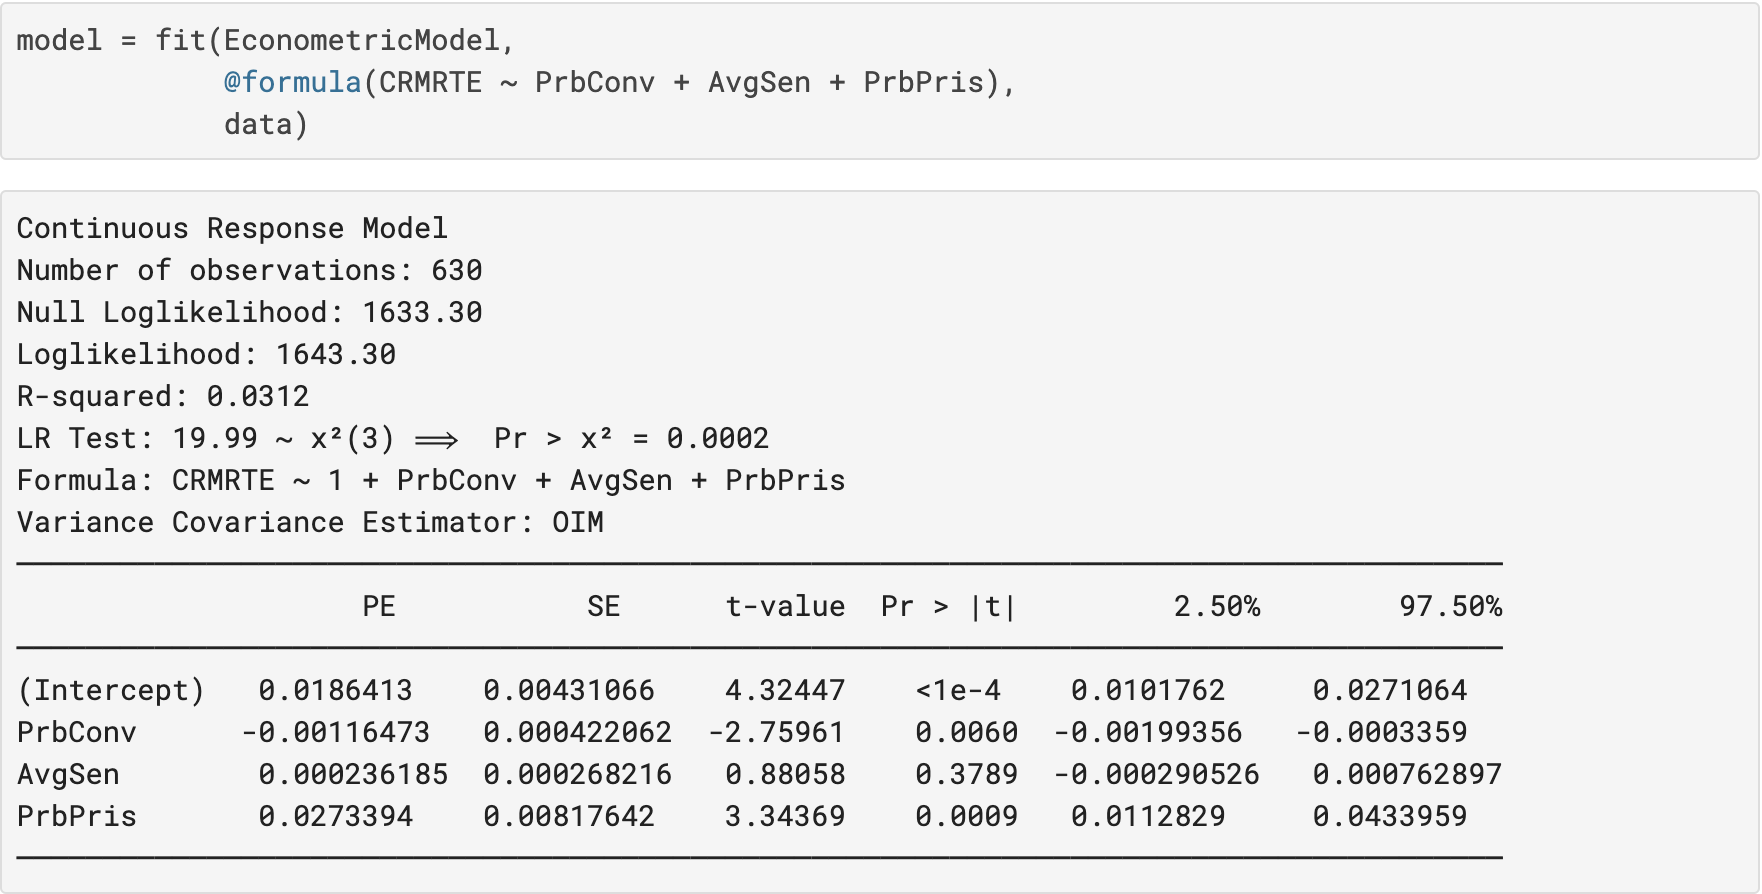
\includegraphics[max width=\linewidth,center]{estimator_pooling}
	\caption{Estimation of the pooling estimator}
	\label{estimator_pooling}
\end{figure}

\begin{figure}[hbpt]
    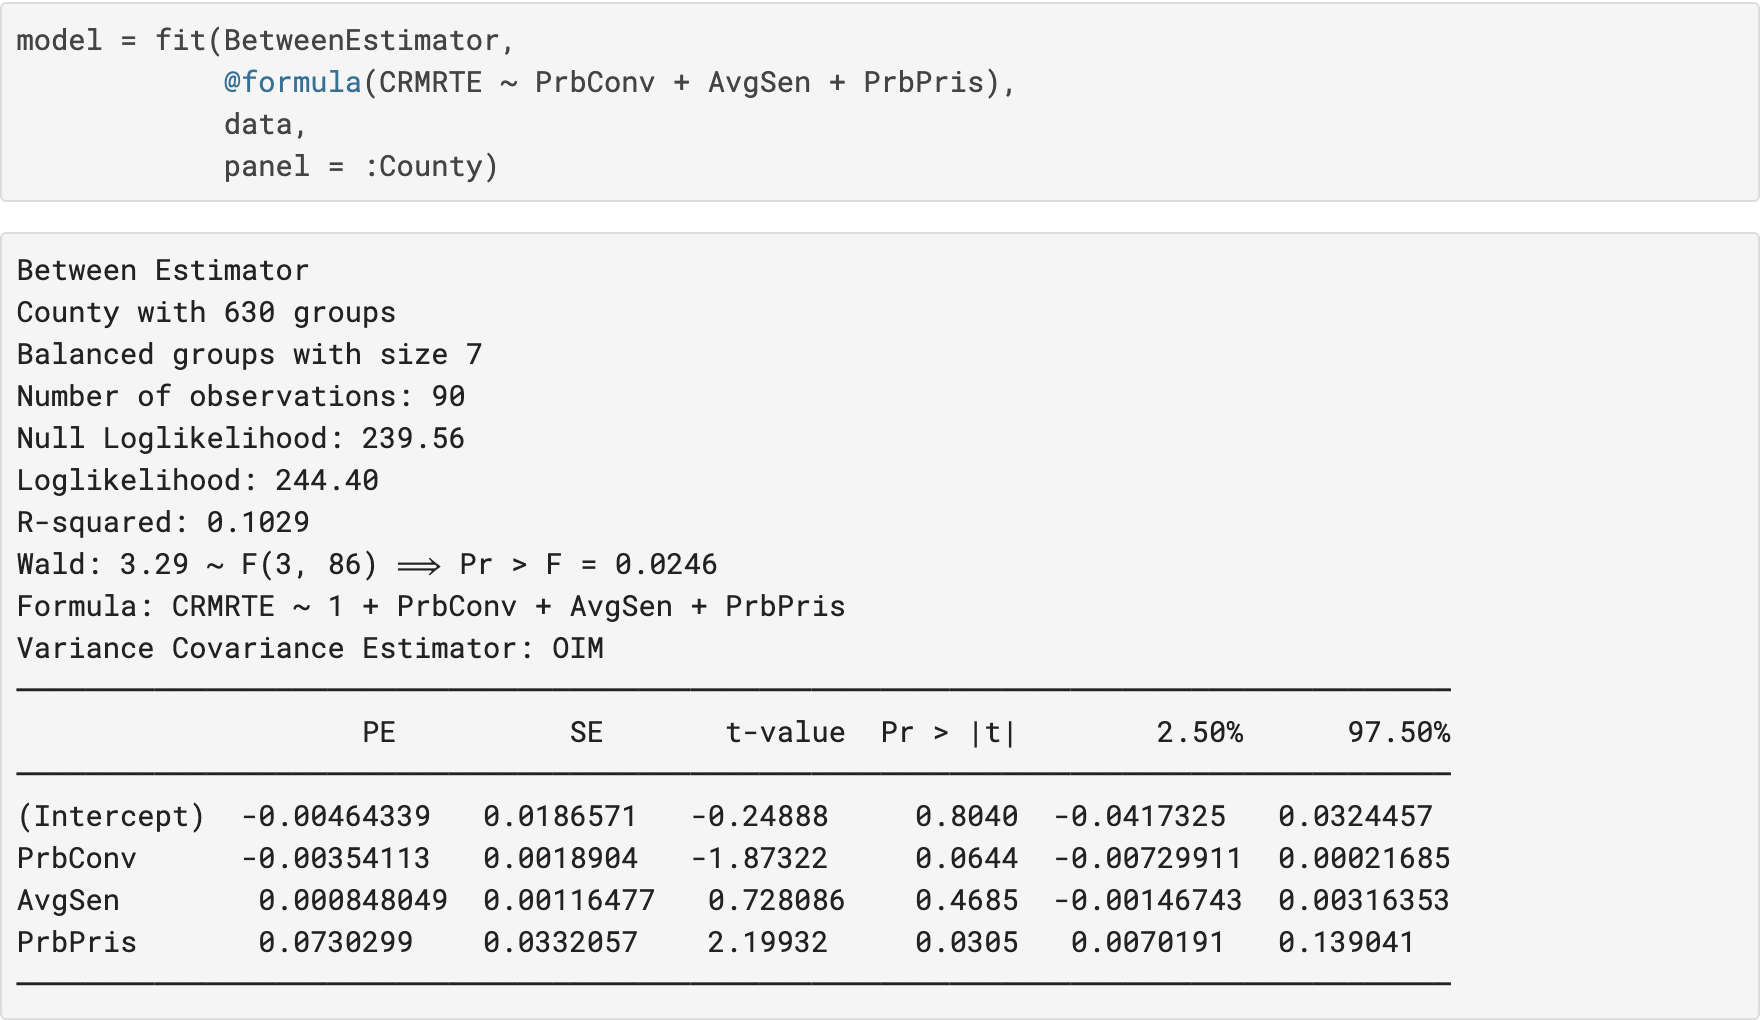
\includegraphics[max width=\linewidth,center]{estimator_between}
	\caption{Estimation of the between panel estimator}
	\label{estimator_between}
\end{figure}

The fixed effects model or within estimator can be estimated as in figure \vref{withinmodel} which estimates the panel effects and the two-ways fixed effects model (i.e., fixed effects for time dimension as well). Table \vref{withinres} shows the estimated 95\% confidence intervals using Econometrics.jl, Stata, and R's plm package.

\begin{figure}[hbpt]
	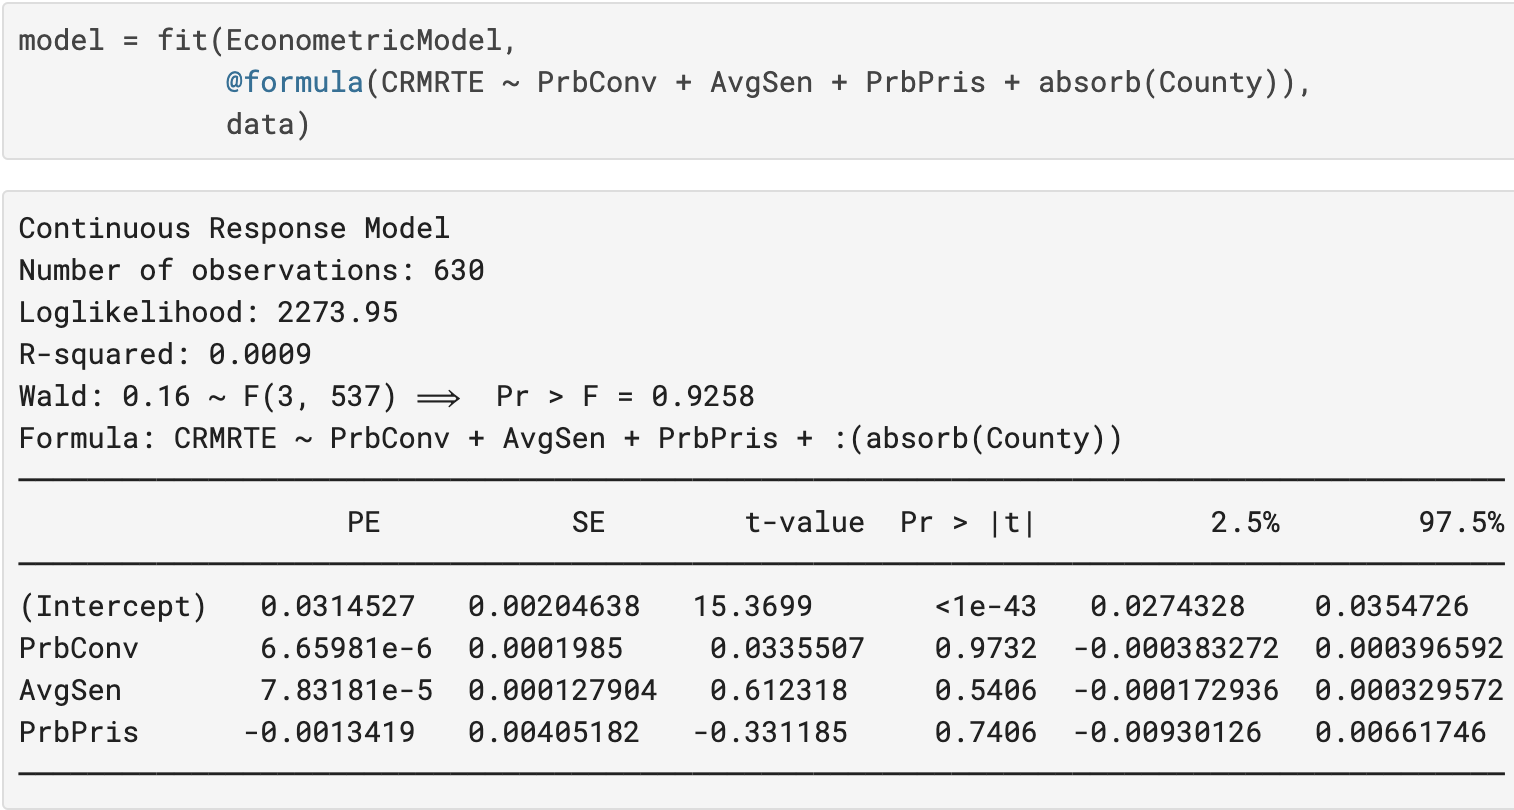
\includegraphics[max width=\linewidth,center]{estimator_within}
	\caption{Estimation of the within estimator}
	\label{withinmodel}
\end{figure}

\begin{figure}[hbpt]
	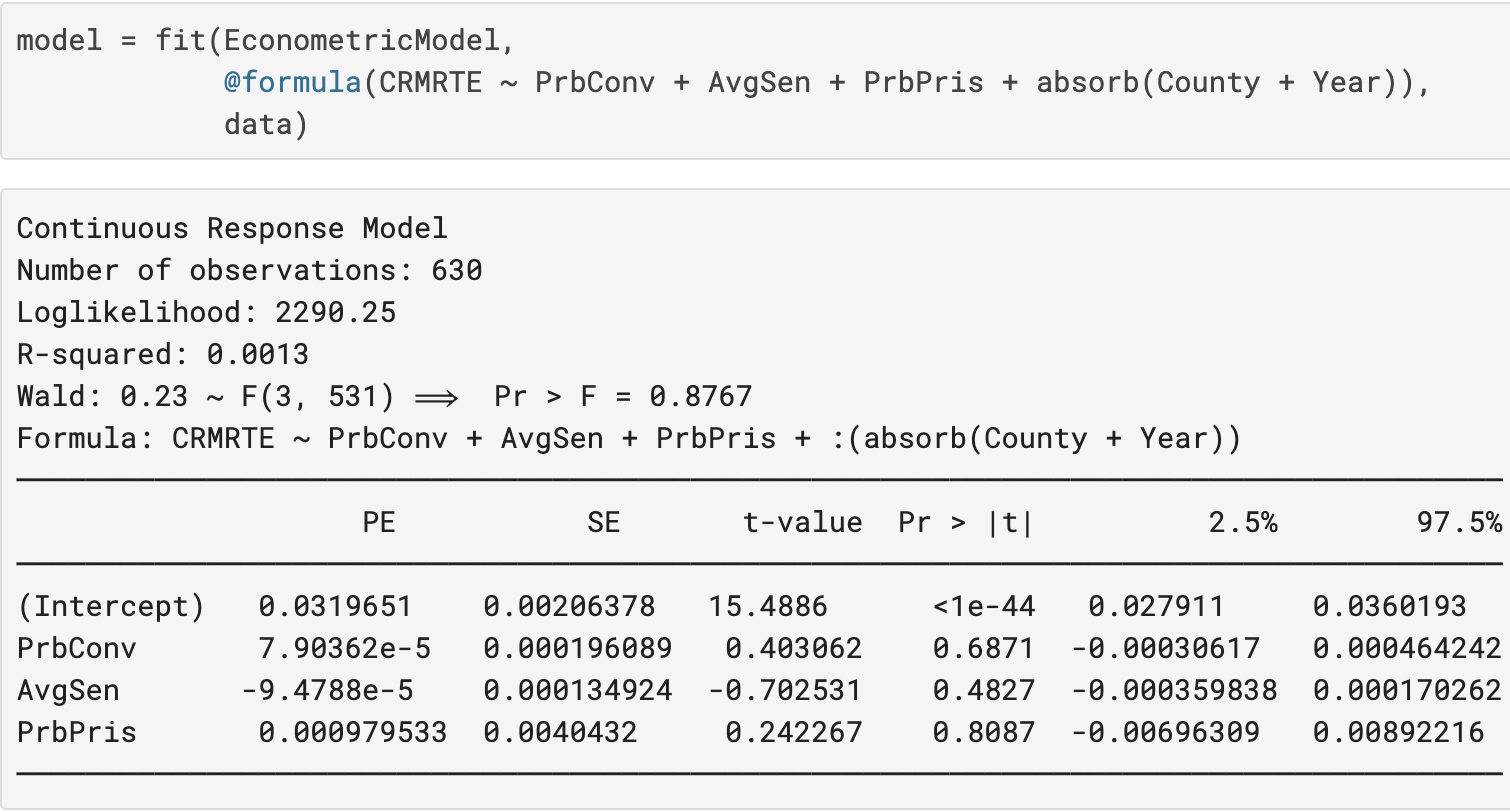
\includegraphics[max width=\linewidth,center]{estimator_within2}
	\caption{Estimation of the within estimator with multiple fixed effects}
	\label{within2model}
\end{figure}

The random effects model can be estimated with similar syntax by including the \textit{PID} (panel identifier) and \textit{TID} (temporal identifier) tags such as in figure \vref{random} which shows estimating a random effects model as well as its instrumental variables counterpart. Table \vref{xtregres} shows the estimated 95\% confidence intervals using Econometrics.jl, Stata's reghdfe module, and R's plm package.

\begin{figure}[hbpt]
	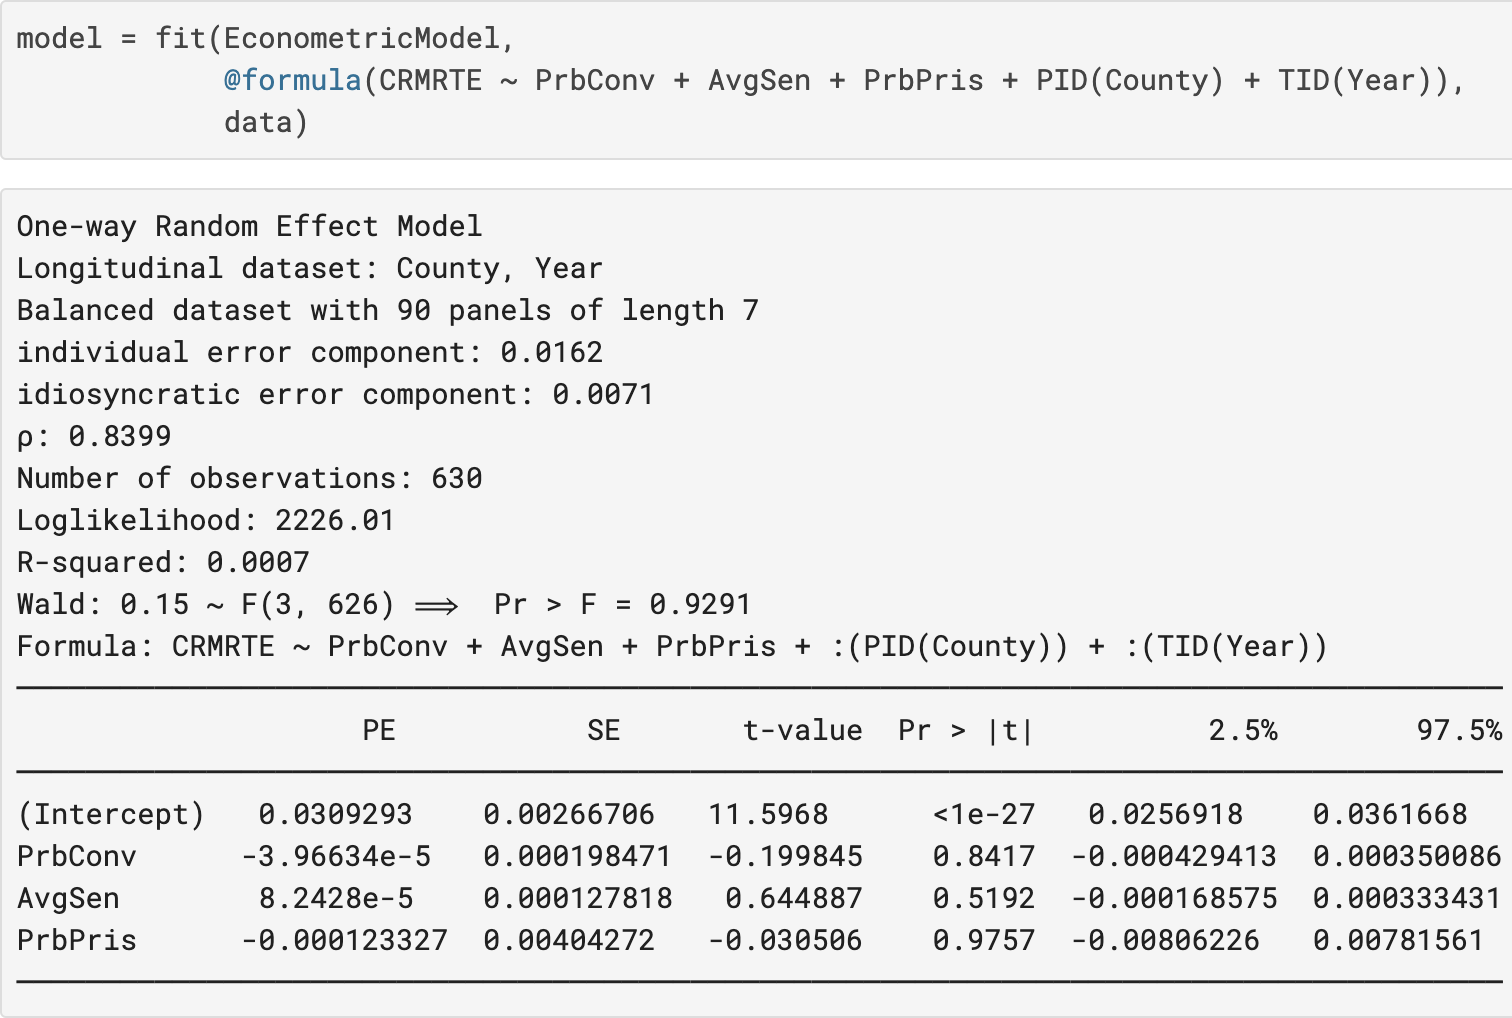
\includegraphics[max width=\linewidth,center]{estimator_re}
	\caption{Estimation of the random effects model}
	\label{random}
\end{figure}

The sysdsn1 Stata example health insurance data set is used to illustrate the multinominal logistic regression when the response is nominal as seen in figure \vref{mlogit}. A comparison with the estimates for the 95\% confidence intervals between Econometrics.jl and Stata is shown in table \vref{mlogitres}.

\begin{figure}[hbpt]
	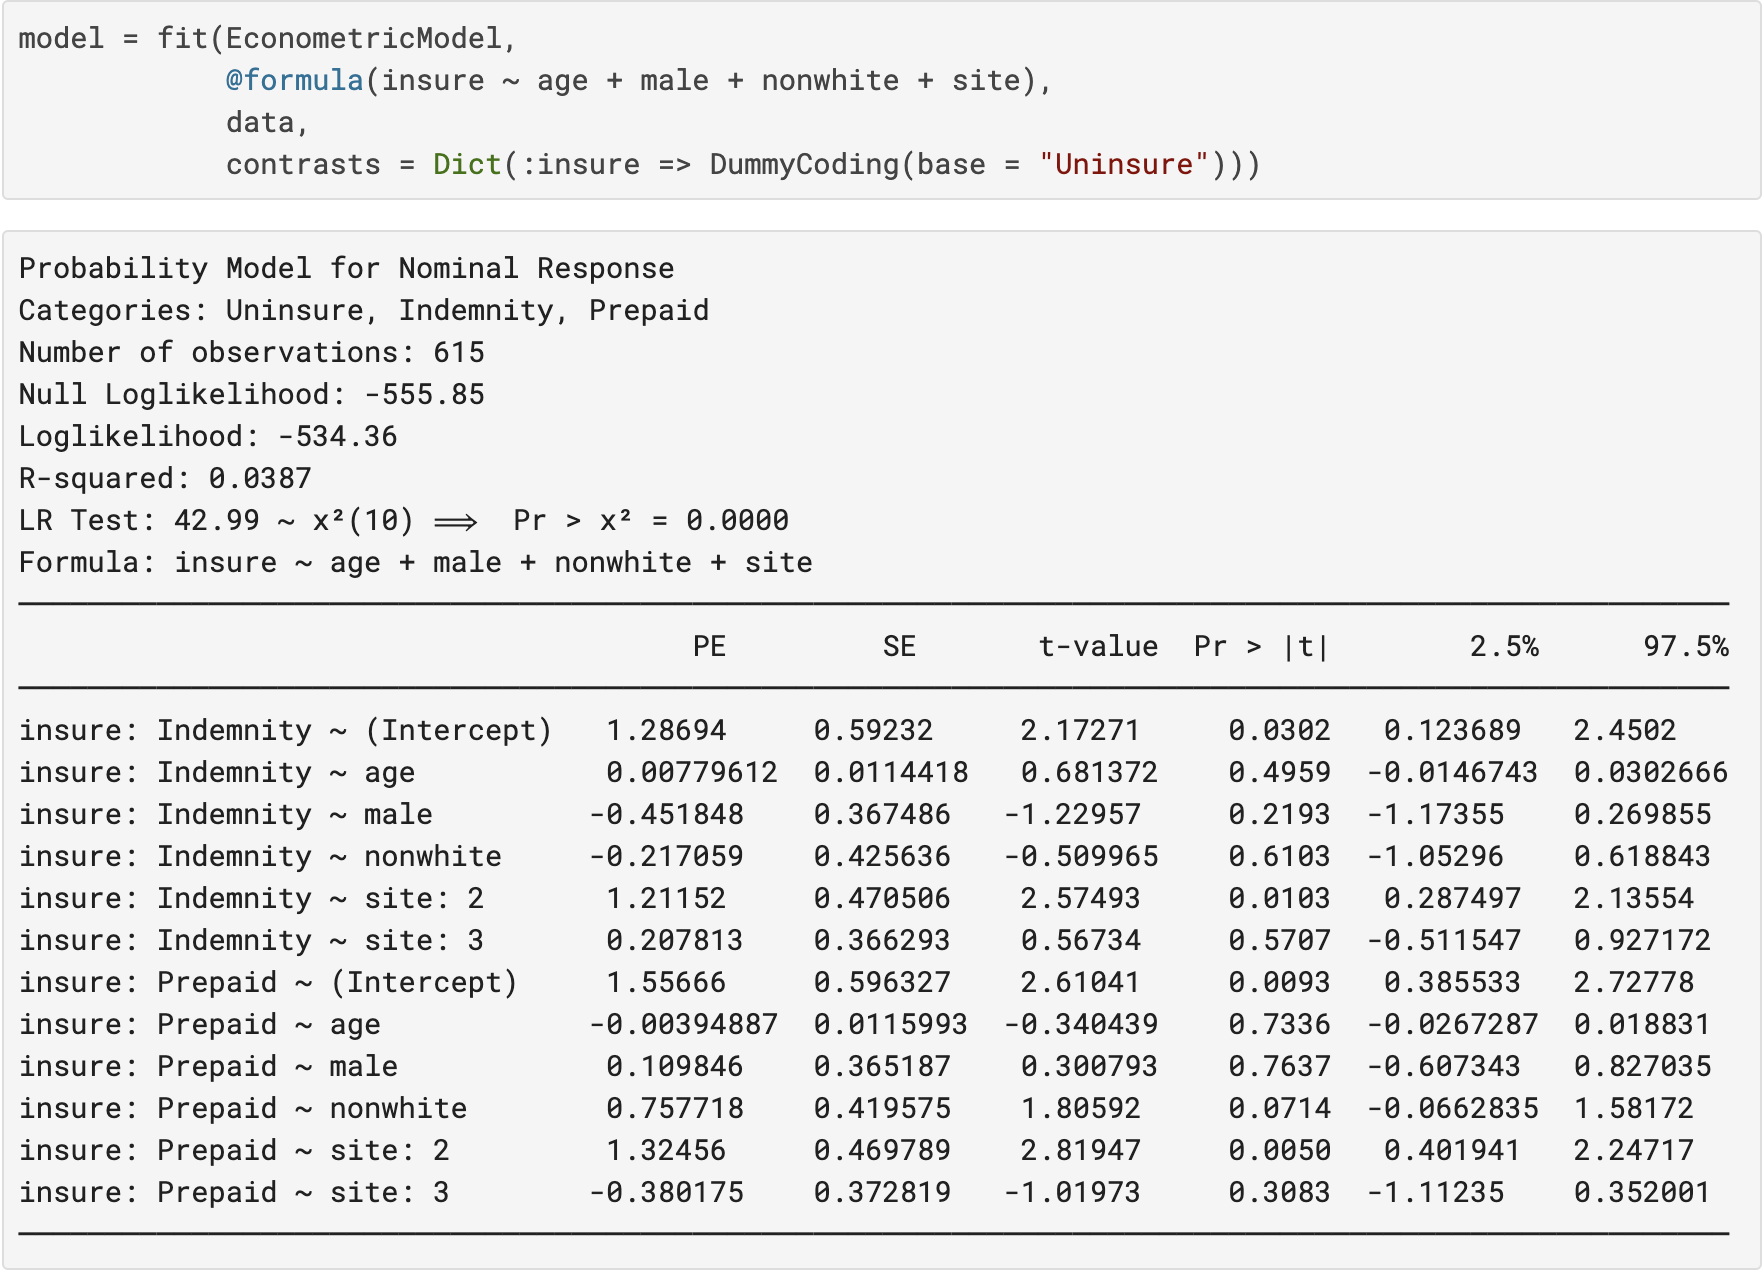
\includegraphics[max width=\linewidth,center]{estimator_mlogit}
	\caption{Estimation of the multinomial logistic regression}
	\label{mlogit}
\end{figure}

The fullauto Stata example automobile models data set is used to illustrate the proportional ordinal logistic regression when the response is ordinal as seen in figure \vref{ologit}. A comparison with the estimates for the 95\% confidence intervals between Econometrics.jl, Stata, and R's MASS is shown in table \vref{ologitres}.

\begin{figure}[hbpt]
	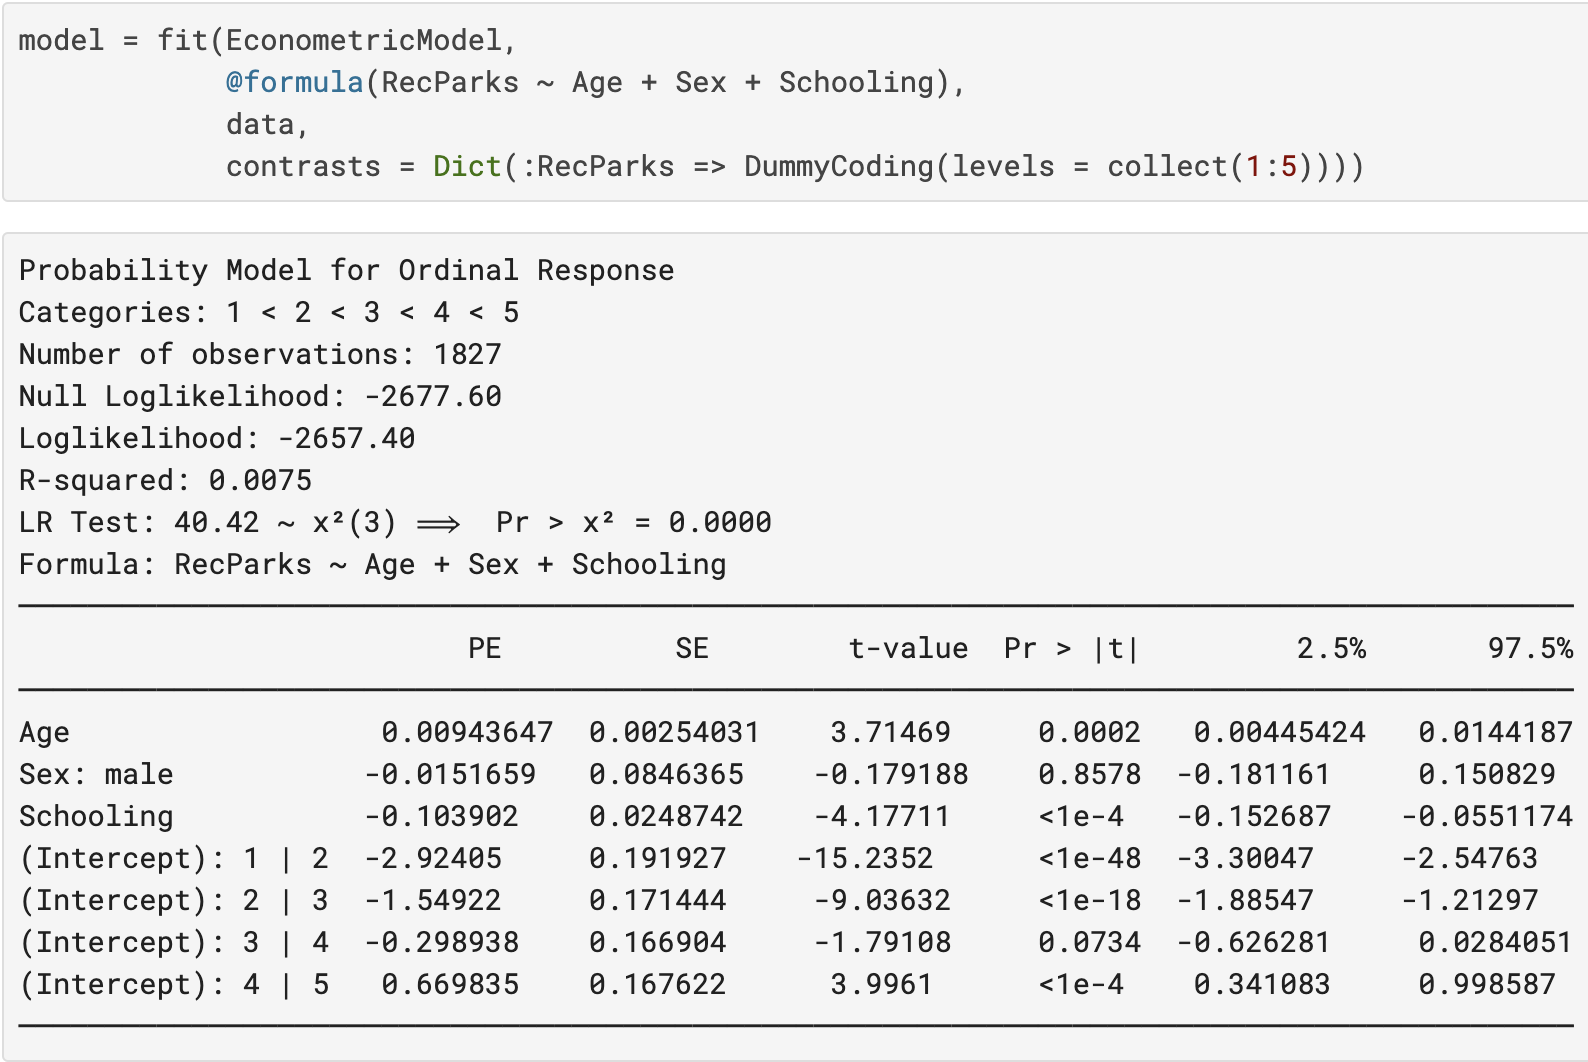
\includegraphics[max width=\linewidth,center]{estimator_ologit}
	\caption{Estimation of the proportional odds logistic regression}
	\label{ologit}
\end{figure}

\subsection{Design Decisions}

Statistical software developers play a very powerful role in shaping culture and norms. For example, whether to default to maximum likelihood estimation (MLE) or restricted maximum likelihood estimation (REML), can shape not only choices by practitioners, but by stakeholders, regulatory agencies, and expected components for reports. These changes may be good or bad depending on the case. For example, advances in econometrics are rarely widely adopted without buy-in from software developers. The following discussions will survey survey some of the decisions relevant to \textit{Econometrics.jl}.

Should software be dummy-proof? Many times software developers have to choose between exposing users to make mistakes on their own volition or put safeguard against potential misuses by restricting behavior that may be correct under rare scenarios. For example, a basic tool might allow users to mix and match link and distributions in a GLM settings even if the combinations are nonsensical. A safer approach would be to restrict combinations to those ``safe'' combinations such as distributions with canonical links. The trade-off occurs when users may encounter a specification that while uncommon it may be the correct one for that particular model. Currently, \textit{Econometrics.jl} takes a conservative approach that provides ``dummy-proof'' experience as well as ease of use. For example, rather than requiring users to specify the model, the estimator is inferred based on the type of the response and information provided. Other examples of this approach include making model statistics such as promoting the coefficient of determination to a pseudo-version for non-linear models (a generalization of the linear case), but providing a \textit{not a number} (NaN) value for instrumental variable models or those that do not include an intercept. Similarly, the software will promote terms to full rank as required and inform of the behavior.

Software analysis should always include diagnostics and tools to make it easier for dissemination. Many tests and diagnostics are applicable to a wide set of implementations. The best manner to make these available and for these to ``play nicely'' with one another is to have an effective API. Sadly, the Julia ecosystem has yet to experience wide adoption of this pattern. For example, packages might need to access components for computing a test or providing some estimates such as variance covariance estimates. The test might include components such as the residual degrees of freedom, the information matrix, residuals, and score. Many implementations might access internals of one particular implementation and compute these such as obtaining the model matrix, response and coefficients to compute the residuals. This behavior would produce incorrect estimates in cases of instrumental variable as the fitted / linear projection should not use the model matrix, but replace the projection of endogenous features with their actual values. A better approach would be to request the response and fitted values to compute the residuals. This approach is less prone to errors, but it can be more robust by calling residuals directly. Specifying precise components can alleviate risk of errors or relying on assumptions such as whether the components are weighted or should be weighted for the procedure.

Various decisions are software specific with asymptotic justification, but significant finite-sample consequences. Software may differ on whether to report statistics using finite-sample statistics (t-distribution, F-distribution) or asymptotic equivalent counterparts (Normal, Chi squared). These tend to have negligible effect in most applications, but other decisions such as degrees of freedom may have larger consequences. For example, software may differs on how it computes the degrees of freedom for instrumental variables or absorbed variables depending on the context (e.g., main regression or auxiliary regression for estimating error components). Refinements and robustness checks can also contribute to a better analysis such as verifying gaps for time variant operations such as first-difference or purging singletons and other degree of freedom adjustments à la \cite{Singletons}.

\subsection{Best Practices}

\textit{Econometrics.jl} adopts the best practices standards for open-source statistical software. These include adhering to semantic versioning (semver) for descriptive versioning, continuous integration for development, software validation through a comprehensive code coverage and test suite, and lastly online hosted documentation for the public API.

\section{Conclusion}

\textit{Econometrics.jl} is a new addition to the Julia ecosystem that brings highly demanded functionality concerning longitudinal estimators and discrete choice models. This study serves as a complement to the software documentation providing context to the development, design considerations, and roadmap of the project. A philosophical motivation for the project is to make econometrics accessible to practitioners not only through functionality, but transparency in the code readability, replicability, and correctness. For example, transparent well-written code is easier to maintain, inspect / audit, and can be useful for learning and teaching.

Community contributions and feedback are highly encouraged in order to best continue developing the project. The release will be available at the Github repository and licensed under a permissive license.

\vfill

% **************GENERATED FILE, DO NOT EDIT**************

\bibliographystyle{juliacon}
\bibliography{ref.bib}


\appendix
\onecolumn
\begin{table}[hbpt]
    \caption{Pooling and Between Estimators}
    \label{poberes}
    \begin{threeparttable}
    \begin{tabularx}{\textwidth}{Y Y c c c c c c}
    \toprule
    Model & Parameter & \multicolumn{2}{c}{Econometrics.jl} & \multicolumn{2}{c}{Stata} & \multicolumn{2}{c}{R (plm)} \\
    \midrule
    \multirow{4}{*}{Pooling} & Intercept & 0.0102 & 0.0271 & 0.0102 & 0.0271 & 0.0102 & 0.0271 \\
    & PrbConv & -0.0020 & -0.0003 & -0.0020 & -0.0003 & -0.0020 & -0.0003 \\
    & AvgSen & -0.0003 & 0.0008 & -0.0003 & 0.0008 & -0.0003 & 0.0008 \\
    & PrbPris & 0.0113 & 0.0434 & 0.0113 & 0.0434 & 0.0113 & 0.0434 \\
    \midrule
    \multirow{4}{*}{Between} & Intercept & -0.0417 & 0.0324 & -0.0417 & 0.0324 & -0.0412 & 0.0319 \\
    & PrbConv & -0.0073 & 0.0002 & -0.0073 & 0.0002 & -0.0072 & 0.0002 \\
    & AvgSen & -0.0015 & 0.0032 & -0.0015 & 0.0032 & -0.0014 & 0.0031 \\
    & PrbPris & 0.0070 & 0.1390 & 0.0070 & 0.1390 & 0.0079 & 0.1381 \\
    \bottomrule
    \end{tabularx}
    \begin{tablenotes}
        \footnotesize
        \item Confidence intervals at the 95\% level using the observed information matrix variance covariance estimator.
    \end{tablenotes}
    \end{threeparttable}
\end{table}
\begin{table}[hbpt]
    \caption{Absorbing Panel or Panel and Temporal Indicators}
    \label{withinres}
    \begin{threeparttable}
    \begin{tabularx}{\textwidth}{Y Y c c c c c c}
    \toprule
    Model & Parameter & \multicolumn{2}{c}{Econometrics.jl} & \multicolumn{2}{c}{Stata (reghdfe)} & \multicolumn{2}{c}{R (plm)} \\
    \midrule
    \multirow{4}{*}{Within PID} & Intercept & 0.0274 & 0.0355 & 0.0274 & 0.0355 &  &  \\
    & PrbConv & -0.0004 & 0.0004 & -0.0004 & 0.0004 & -0.0004 & 0.0004 \\
    & AvgSen & -0.0002 & 0.0003 & -0.0002 & 0.0003 & -0.0002 & 0.0003 \\
    & PrbPris & -0.0093 & 0.0066 & -0.0093 & 0.0066 & -0.0093 & 0.0066 \\
    \midrule
    \multirow{4}{*}{Within PTID} & Intercept & 0.0279 & 0.0360 & 0.0279 & 0.0360 &  &  \\
    & PrbConv & -0.0003 & 0.0005 & -0.0003 & 0.0005 & -0.0003 & 0.0005 \\
    & AvgSen & -0.0004 & 0.0002 & -0.0004 & 0.0002 & -0.0004 & 0.0002 \\
    & PrbPris & -0.0070 & 0.0089 & -0.0070 & 0.0089 & -0.0069 & 0.0089 \\
    \bottomrule
    \end{tabularx}
    \begin{tablenotes}
        \footnotesize
        \item Confidence intervals at the 95\% level using the observed information matrix variance covariance estimator.
    \end{tablenotes}
    \end{threeparttable}
\end{table}
\begin{table}[hbpt]
    \caption{Random Effects and Instrumental Variables}
    \label{xtregres}
    \begin{threeparttable}
    \begin{tabularx}{\textwidth}{Y Y c c c c c c}
    \toprule
    Model & Parameter & \multicolumn{2}{c}{Econometrics.jl} & \multicolumn{2}{c}{Stata} & \multicolumn{2}{c}{R (plm)} \\
    \midrule
    \multirow{4}{*}{Random} & Intercept & 0.0257 & 0.0362 & 0.0257 & 0.0362 &  &  \\
    & PrbConv & -0.0004 & 0.0004 & -0.0004 & 0.0003 & -0.0004 & 0.0004 \\
    & AvgSen & -0.0002 & 0.0003 & -0.0002 & 0.0003 & -0.0002 & 0.0003 \\
    & PrbPris & -0.0081 & 0.0078 & -0.0080 & 0.0078 & -0.0093 & 0.0066 \\
    \midrule
    \multirow{3}{*}{IV Random} & Intercept & -0.0097 & 0.0852 & -0.0096 & 0.0851 & -0.0096 & 0.0851 \\
    & PrbConv & -0.0004 & 0.0004 & -0.0004 & 0.0004 & -0.0004 & 0.0004 \\
    & AvgSen & -0.0059 & 0.0045 & -0.0059 & 0.0045 & -0.0059 & 0.0045 \\
    \bottomrule
    \end{tabularx}
    \begin{tablenotes}
        \footnotesize
        \item Confidence intervals at the 95\% level using the observed information matrix variance covariance estimator.
    \end{tablenotes}
    \end{threeparttable}
\end{table}
\begin{table}[hbpt]
    \caption{Multinomial Logistic Regression}
    \label{mlogitres}
    \begin{tabularx}{\textwidth}{Y Y c c c c}
    \toprule
    Response & Parameter & \multicolumn{2}{l}{Econometrics.jl} & \multicolumn{2}{c}{Stata} \\
    \midrule
    \multirow{6}{*}{Indemnity} & (Intercept) & -0.3753 & 0.9148 & -0.3740 & 0.9134 \\
    & Age & -0.0239 & 0.0004 & -0.0239 & 0.0004 \\
    & Gender: Male & 0.1635 & 0.9599 & 0.1643 & 0.9591 \\
    & Nonwhite & 0.5107 & 1.4389 & 0.5116 & 1.4380 \\
    & Site: 2 & -0.2998 & 0.5258 & -0.2989 & 0.5250 \\
    & Site: 3 & -1.0356 & -0.1404 & -1.0347 & -0.1412 \\
    \midrule
    \multirow{6}{*}{Prepaid} & (Intercept) & -2.4502 & -0.1237 & -2.4479 & -0.1260 \\
    & Age & -0.0303 & 0.0147 & -0.0302 & 0.0146 \\
    & Gender: Male & -0.2698 & 1.1736 & -0.2684 & 1.1721 \\
    & Nonwhite & -0.6188 & 1.0530 & -0.6172 & 1.0513 \\
    & Site: 2 & -2.1356 & -0.2875 & -2.1338 & -0.2894 \\
    & Site: 3 & -0.9272 & 0.5115 & -0.9257 & 0.5101 \\
    \bottomrule
    \end{tabularx}
\end{table}
\begin{table}[hbpt]
    \caption{Parallel Ordinal Logistic Regression}
    \label{ologitres}
    \begin{tabularx}{\textwidth}{Y c c c c c c}
    \toprule
    Parameter & \multicolumn{2}{c}{Econometrics.jl} & \multicolumn{2}{c}{Stata} & \multicolumn{2}{c}{R’s MASS} \\
    \midrule
    Foreign & 1.3168 & 4.4768 & 1.3472 & 4.4464 & 1.4111 & 4.5293 \\
    Length & 0.0374 & 0.1282 & 0.0383 & 0.1274 & 0.0395 & 0.1292 \\
    MPG & 0.0900 & 0.3716 & 0.0927 & 0.3689 & 0.0986 & 0.3781 \\
    (Intercept): Poor | Fair & 6.8343 & 29.0206 & 7.0473 & 28.8076 &  &  \\
    (Intercept): Fair | Average & 8.6814 & 31.0487 & 8.8962 & 30.8340 &  &  \\
    (Intercept): Average | Good & 10.6949 & 33.5117 & 10.9140 & 33.2926 &  &  \\
    (Intercept): Good | Excellent & 12.9204 & 36.4639 & 13.1465 & 36.2378 &  & \\
    \bottomrule
\end{tabularx}
\end{table}

\end{document}

% Inspired by the International Journal of Computer Applications template
